
\documentclass[xetex,professionalfont]{beamer}

\usepackage{amsmath}

\usepackage{mathtools}

\usepackage{amssymb}

\usepackage{xspace}

\usepackage{booktabs}


\usepackage{fontspec}
\setmonofont[Scale=0.7]{Droid Sans Mono} %

\usepackage[caption=false]{subfig}
\captionsetup{belowskip=0pt,aboveskip=0pt}

\usepackage{csquotes}


\usepackage[english]{babel}


\usepackage{tikz}


\hypersetup{pdftitle={DLVC Introduction},pdfsubject={},pdfauthor={Christopher Pramerdorfer},colorlinks,urlcolor=tuwcvl_cvl_blue,linkcolor=tuwcvl_textlight}


\let\oldemph\emph
\renewcommand\emph[1]{\textcolor{tuwcvl_cvl_blue}{#1}}

\usefonttheme[onlymath]{serif}

\usetheme{dlvc}



\newcommand{\ie}{\mbox{i.e.}\xspace} %
\newcommand{\eg}{\mbox{e.g.}\xspace} %

\DeclareMathOperator*{\argmin}{arg\,min}
\DeclareMathOperator*{\argmax}{arg\,max}

\newcommand{\NN}{\mathbb{N}}
\newcommand{\ZZ}{\mathbb{Z}}
\newcommand{\QQ}{\mathbb{Q}}
\newcommand{\RR}{\mathbb{R}}

\renewcommand{\vec}[1]{\ensuremath{\mathbf{#1}}}

\newcommand{\va}{\vec{a}}
\newcommand{\vb}{\vec{b}}
\newcommand{\vc}{\vec{c}}
\newcommand{\ve}{\vec{e}}
\newcommand{\vr}{\vec{r}}
\newcommand{\vs}{\vec{s}}
\newcommand{\vt}{\vec{t}}
\newcommand{\vu}{\vec{u}}
\newcommand{\vv}{\vec{v}}
\newcommand{\vw}{\vec{w}}
\newcommand{\vx}{\vec{x}}
\newcommand{\vy}{\vec{y}}
\newcommand{\vz}{\vec{z}}

\makeatletter
\let\@@magyar@captionfix\relax
\makeatother


\title{Deep Learning for Visual Computing}
\subtitle{Introduction}
\author{Christopher Pramerdorfer}
\institute{Computer Vision Lab, TU Wien}

\begin{document}


\begin{frame}
\maketitle
\end{frame}


{
\setbeamertemplate{footline}{}
\begin{frame}

\begin{tikzpicture}[remember picture,overlay]
\fill[white] (current page.north west) rectangle (current page.south east);
\end{tikzpicture}

\begin{center}
  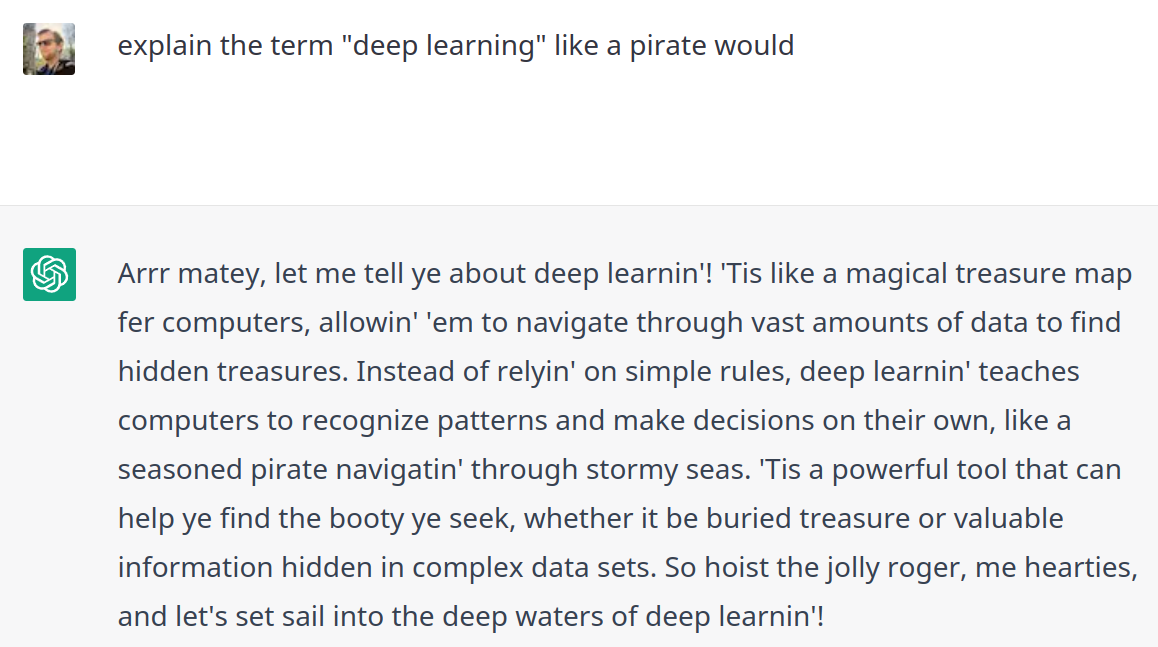
\includegraphics[width=10cm]{images/openai}
\end{center}

\end{frame}
}


\begin{frame}
  \frametitle{Motivation}

\emph{AI}
\begin{itemize}
  \item Is everywhere
  \item Is here to stay
\end{itemize}

\bigskip
\emph{Deep learning} is what makes this possible
\begin{itemize}
  \item Has revolutionized computer vision \& machine learning
  \item Beats humans at many complex tasks
  \item Enables novel applications (e.g.~ChatGPT, StableDiffusion)
\end{itemize}

\end{frame}


\begin{frame}
\frametitle{Goals}

Goal is to teach you
\begin{itemize}
    \item How deep learning works
    \item How it can be used to solve various problems
    \item How to apply deep learning in practice
    \item How it is related to machine learning \& computer vision
\end{itemize}

\end{frame}


\begin{frame}
\frametitle{Lecture Topics}

Introduction
\begin{itemize}
    \item Recap of computer vision and machine learning
    \item Feedforward neural networks, backpropagation
\end{itemize}

\bigskip

Deep learning
\begin{itemize}
    \item Convolutional neural networks
    \item Generative neural networks
    \item Transformers
    \item Ethical apsects \& XAI
\end{itemize}

\end{frame}


\begin{frame}
  \frametitle{Lecture}
  Usually Tuesdays, 15:15 to 16:45 at EI 1 (here)
  \begin{itemize}
    \item Changes will be communicated via TISS
  \end{itemize}
  \bigskip
  Slides will be available on TUWEL
  \begin{itemize}
    \item Usually the morning before the lecture
  \end{itemize}
\end{frame}


\begin{frame}
  \frametitle{Assignments}
  Apply what you've learned in the lecture

  \bigskip
  Three assignments in groups of two (no exceptions)
  \begin{itemize}
    \item Code in Python 3 and \href{https://pytorch.org/}{PyTorch} (reference available)
    \item Write short report explaining what you did
  \end{itemize}

  \bigskip
  Code at home, in the cloud, or on our servers (details later)

  \bigskip
  Hand in via TUWEL
\end{frame}


\begin{frame}
  \frametitle{Initial Assignment}
  Initial assignment
  \begin{itemize}
    \item \emph{Must be handed in until March 14}
    \item Done solo (before group registration)
    \item Required for positive grade
    \item People who submit will get a grade
  \end{itemize}

  \bigskip
  If you don't want to continue
  \begin{itemize}
    \item Unsubscribe from course today
    \item Don't hand in the initial assignment
  \end{itemize}
\end{frame}


\begin{frame}
\frametitle{Prerequisites}

Studies
\begin{itemize}
  \item Be a MSc or PhD student
\end{itemize}

\bigskip

Skills
\begin{itemize}
  \item Proficiency in Python
  \item Basic knowledge of statistics, linear algebra, calculus
  \item Basic knowledge of image processing and machine learning
\end{itemize}
\end{frame}


\begin{frame}
\frametitle{Grading}

Assignments (50\%)
\begin{itemize}
  \item All assignments must be positive (50\% or more points)
  \item Penalties for late submissions (up to one week)
\end{itemize}

\bigskip

Written exam (50\%)
\begin{itemize}
    \item 60 minutes
    \item List of questions available
    \item German or English
\end{itemize}

\bigskip

Both must be positive to pass

\end{frame}


\begin{frame}
  \frametitle{Registration}
  Register via TISS until tomorrow at 23:00

  \bigskip
  Course is completely full
  \begin{itemize}
    \item If you can't make it to lectures, please unsubscribe
    \item There will be no recordings or video streams
  \end{itemize}

  \bigskip
  Current registration status is temporary
  \begin{itemize}
    \item Priority is MSc > PhD > BSc
    \item Registrations will be finalized after deregistration period
  \end{itemize}
\end{frame}


\begin{frame}
  \frametitle{Support}
  Support
  \begin{itemize}
    \item After lectures
    \item Via TUWEL course forums
  \end{itemize}
\end{frame}


\begin{frame}
\frametitle{Questions}

\begin{center}
Questions?
\end{center}

\end{frame}

\end{document}
